\section{Algorithm}

\subsection{Problem Definition and Assumptions}
We define a goal region $G^{\textrm{full}}$ as a discretized set of initial object poses on the conveyor belt that the robot can perceive when the object comes in its field of view. Given a home configuration for the robot $s_{\textrm{home}}$, we want to be able to plan for any goal pose $g_{\textrm{init}}$ in bounded time $t_{\textrm{bound}}$. The perception system is setup such that it sends updated pose estimates on the fly during execution as it gets better estimates over time. Given any current state of the robot during execution $s_{\textrm{start}}$, the planner should be able to replan from $s_{\textrm{start}}$ to any subsequent goal $g_{\textrm{next}}$.

We make the following assumptions about the system.
\begin{itemize}
\item $G^{\textrm{full}}$ would accommodate for an error $\epsilon$ in the initial pose estimate $g_{\textrm{init}}$ of the perception system. Each subsequent estimate $g_{\textrm{next}}$ will be within the $\epsilon$ window around $g_{\textrm{init}}$ (in retrospect because the conveyor is moving).
\item We assume that all $\forall g \in G^{\textrm{full}}$, there exists a path from $s_{\textrm{home}}$ to $g$ and we can find it in finite preprocessing time (not sure about this one)
\item We assume that the reachable set of goals for a state on a path is a subset of the reachable set of every other state on that path that exists before it.
\item There exists a replan cutoff time $\Trc$ from when the robot starts moving, after which the planner does not accept more replanning requests.
\item We assume that before $\Trc$, the environment is static. In other words the moving target object cannot collide with the robot during that time.
\end{itemize}

\subsection{Properties}
\begin{itemize}
\item The planning time for each planning/replanning request is bounded ($t_{\textrm{bound}}$)
\item We discretize the trajectories with the resolution $\delta t$. The reaction time of the robot to a replanning request is bounded by $t_{\textrm{bound}} + \delta t$
\end{itemize}

\subsection{Offline Motion Planner}
In this section we will describe the motion planner that is used in the \textsc{PlanPath()} and \textsc{PlanPathUsingRootPath()} functions in Algs.~\ref{alg:3} and~\ref{alg:4}. We use a heuristic search based planning approach with motion primitives (cite papers here). There are a few advantages of this approach for our particular problem.
\begin{itemize}
    \item It can elegantly handle under-defined goals. We define a goal as a 6DOF grasp pose for the goal object. The goal is underdefined as there is a redundant degree of freedom of the robot and also because the grasping time is not specified.
    \item We make use of a set of predefined motion primitives and dynamically generated motion primitives which can be computed such that the kinodynamic constraints of the robot are respected. These primitives are used to generate an implicit graph which is searched by a heuristic search-based planner to compute a plan
    \item We can design informative heuristic functions to speed up the search
    \item We use an existing search-based algorithm e-graphs (cite here) that reuses past experiences and significantly reduces planning times for repetitive tasks
\end{itemize}


\subsubsection{State Space and Graph Construction}

Let $G = (S,E)$ denote an implicit directed graph that we construct, where $S$ denotes the states on $E$ denotes the directed edges that define the transition between this states. A state $s$ in $S$ is uniquely defined by the tuple ($\mathcal{X},t$), $\mathcal{X}$ being an $n$-tuple representing joint angles ($\theta_0, \theta_1, ..., \theta_n$) for an $n$-DOF robot arm and $t$ is the time associated with $s$.
The edges $E$ corresponds to motion primitives which are short kinodynamically feasible motions that the robot can execute. We use two sets of motion primitives, \textit{predefined} and \textit{dynamic}. The predefined set of primitives are small individual joint movements in either direction as well as \textit{wait} actions i.e $(\pm \Delta \theta_0, \pm \Delta \theta_1, ..., \pm \Delta \theta_n, \Delta t)$. For each joint motion primitive $\pm \theta_i$, we compute its duration by using a nominal constant velocity profile for that joint. While a plan generated on $G$ is not guaranteed to respect the acceleration limits of the robot, in our experience, the trajectory execution error seldom occured. Neverthelessm, we will elaborate in the experiments section how our replanning framework can handle the execution errors.

The dynamic primitives are generated by using a Jacobian pseudo inverse based control low. The inverse velocity kinematics of the manipulator is given by
\begin{center}
$\dot{\mathcal{X}} = J^{-1}(\mathcal{X})\dot{q}$
\end{center}

where $J^{-1}$ is the Jacobian pseudo inverse and $\dot{q}$ represents the desired task space velocity of the end-effector. $\dot{q}$ is computed such that the end-effector minimises distance to the grasp pose and once the gripper encloses the object, it moves along with the object until the gripper is closed. The motion generated by the roll out of this control law constitutes the dynamic primitive. The dynamic primitives are only generated when the expanded state is within a threshold distance from the goal. 
\os{add figure showing the dynamic primitive}

\subsubsection{Heuristic Search-based Planning}
We use Weighted A* (WA*) search to find a path from $s_{\textrm{start}}$ to $s_{\textrm{goal}}$ on the graph $G$. WA* is a suboptimal heursitic search that tradesoff optimality and greediness. The search is guided by an efficient and fast to compute heuristic function. The heuristic function that we use has two components, one that tries to intercept the object at the right time and the other guides to the search to correct the orientation when the end-effector approaches the object. The heuristic function is given by

\begin{center}
$h(s,g) = \max (w \cdot t(s,g), \textsc{AngleDiff}(s,g))$
\end{center}

\os{We can talk about the overall suboptimality bound here}

The term $t(s,g)$ is the expected time to intercept the object. It can be analytically computed from the velocities and positions of the target object and the end-effector.
(\os{need a figure to explain it})
\textsc{AngleDiff}($s,g$) gives the the magnitude of angular difference between the end-effector's current pose and target pose in axis-angle form.

\begin{algorithm}
\caption{\textsc{PreprocessMain()}}\label{alg:1}
% Precompute trunks $\{\Pi_{G^{\textrm{full}}}\}$ from $s_{\textrm{home}}$ that cover $G^{\textrm{full}}$
\hspace*{\algorithmicindent} \textbf{Inputs} $s_{\textrm{home}}, G^{\textrm{full}}$ \\
% \hspace*{\algorithmicindent} \textbf{Output} 
\begin{algorithmic}[1]
% \State $\Psi_{\textrm{home}}, G'^{\textrm{full}} \leftarrow$ \textsc{ComputeRootPaths}($s_{\textrm{home}},G^{\textrm{full}}$)
\State \textsc{Preprocess}($s_{\textrm{home}},G^{\textrm{full}},\emptyset$)
\end{algorithmic}
\end{algorithm}

\begin{algorithm}
\caption{\textsc{Preprocess}($s_{\textrm{start}},G^{\textrm{UNCOV}},G^{\textrm{COV}}$)}\label{alg:2}
\begin{algorithmic}[1]
\State $\Psi_{\textrm{work}}, G'^{\textrm{UNCOV}}_{\textrm{work}} \leftarrow$ \textsc{ComputeRootPaths\&GoalRegions}($s_{\textrm{start}},G^{\textrm{UNCOV}}$)

\If {$s_{\textrm{start}} = s_{\textrm{home}}$}
    \State $\Psi_{\textrm{home}} = \Psi_{\textrm{work}}$
\EndIf
% \State $G'^{\textrm{COV}} \leftarrow G'^{\textrm{COV}} \bigcup G^{\textrm{COV}}$
\State $G'^{\textrm{COV}} \leftarrow G^{\textrm{COV}} \cup (G^{\textrm{UNCOV}} - G'^{\textrm{UNCOV}}_{\textrm{work}})$
\If{$t(s_{\textrm{start}}) \geq \Trc$}
    \State \textbf{return} $G'^{\textrm{UNCOV}}_{\textrm{work}}, G'^{\textrm{COV}}$
\EndIf
\For {\textbf{each} $(\Pi_{G_i}, G_i) \in \Psi_{\textrm{work}}$}
% \For {$i \leftarrow$ 1 to $|\{\Pi_{\textrm{work}}\}|$}
    % \State $\Pi_{G_i}, G_i \leftarrow$ \textsc{GetRootPathAndGoalRegion}($s_{\textrm{start}},i$)
    \State $t = \Trc$
    \State $G_i^{\textrm{uncov}} \leftarrow G'^{\textrm{COV}} - G_i$
    \State $G_i^{\textrm{cov}} \leftarrow G_i$

    % {\color{BrickRed}
    % \State $G_i^{\textrm{uncov}} \leftarrow G_i^{\textrm{uncov}} - G_i$
    % \State $G_i^{\textrm{cov}} \leftarrow G_i^{\textrm{cov}} \cup G_i$
    % }
    
    \While{$t \geq t(s_{\textrm{start}})$}
        \State $s \leftarrow$ \textsc{GetState($\Pi_{G_i}, t$)}
        %%%%%%% LATCHING BEGIN
      % {\color{blue}
       \For {\textbf{each} $(\Pi_{G_j}, G_j) \in \Psi_{\textrm{home}}$}
            \If{\textsc{CheckSnap}($s,\Pi_{G_j}$)}
                \State $G_i^{\textrm{uncov}} \leftarrow G_i^{\textrm{uncov}} - G_j$
                \State $G_i^{\textrm{cov}} \leftarrow G_i^{\textrm{cov}} \cup G_j$
            \EndIf
        \EndFor
        % }
        %%%%%%%%% LATCHING END
        \If{$G_i^{\textrm{uncov}} = \emptyset$}
            \State \textbf{break}
        \EndIf
        \State $G_i^{\textrm{uncov}},G_i^{\textrm{cov}} \leftarrow$ \textsc{Preprocess}($s,G_i^{\textrm{uncov}},G_i^{\textrm{cov}}$)
        \If{$G_i^{\textrm{uncov}} = \emptyset$}
            \State \textbf{break}
        \EndIf
        \State $t = t - \delta t$
    \EndWhile
    % \State $(\Pi_i,\Pi_j).s = s$ \Comment{replan state}
\EndFor
\State \textbf{return} $G'^{\textrm{UNCOV}}_{\textrm{work}}, G'^{\textrm{COV}}$

\end{algorithmic}
\end{algorithm}

\begin{algorithm}
\caption{\textsc{Query}($g, \pi_{\textrm{curr}},s_{\textrm{start}}$)}\label{alg:3}  
\begin{algorithmic}[1]
    % {\color{BrickRed}
    \State $\Pi_{\textrm{curr}} \leftarrow$ \textsc{LookupRootPath}($s_{\textrm{start}},g$)
        % \State \textbf{return} $\pi_{\textrm{curr}}$
    \If{$\Pi_{\textrm{curr}} \neq \emptyset$}
        \State $\pi \leftarrow$ \textsc{PlanPathUsingRootPath}($s_{\textrm{start}},g,\Pi_{\textrm{curr}}$)
        \State \textbf{return} $\pi$
    \EndIf
    % }

\State $t = \Trc$
\While{$t \geq t_{\textrm{curr}}$}
    \State $s \leftarrow$ \textsc{GetState}($\pi_{\textrm{curr}}, t$)
    \State $\Pi_{\textrm{next}} \leftarrow$  \textsc{LookupRootPath}($s,g$)
    \If{$\Pi_{\textrm{next}} \neq \emptyset$}
        \State $\pi_{\textrm{next}} \leftarrow$\textsc{PlanPathUsingRootPath}($s_{\textrm{start}},g,\Pi_{\textrm{next}}$)
        \State $\pi \leftarrow$ \textsc{MergePaths}($\pi_{\textrm{curr}},\pi_{\textrm{next}},t$)
        \State \textbf{return} $\pi$
    \EndIf
%%%%%%%%%%%%%%%%LATCHING 
    {\color{blue}
    \State $\Pi_{\textrm{home}} \leftarrow$ \textsc{LookupRootPath}($s_{\textrm{home}},g$)
    \If{$\Pi_{\textrm{home}} \neq \emptyset$}
        \If{\textsc{CheckSnap}($s,\Pi_{\textrm{home}}$)}
            \State $\pi_{\textrm{home}} \leftarrow$\textsc{PlanPathUsingRootPath}($s_{\textrm{start}},g,\Pi_{\textrm{home}}$)
            \State $\pi \leftarrow$ \textsc{MergePathsWithSnap}($\pi_{\textrm{curr}},\pi_{\textrm{home}}, t$)
            \State \textbf{return} $\pi$
        \EndIf
    \EndIf
    }
%%%%%%%%%%%
    \State $t = t - \delta t$
\EndWhile
\State \textbf{return failure}
\end{algorithmic}
\end{algorithm}

\begin{algorithm}
\caption{\textsc{ComputeRootPaths$\&$GoalRegions}($s_{\textrm{start}}, G^{\textrm{UNCOV}}$)}\label{alg:4}
\begin{algorithmic}[1]
\State $\Psi \leftarrow \emptyset$   \Comment{A list of pairs ($\Pi, G)$)}
\State $G'^{\textrm{UNCOV}} \leftarrow \emptyset$
\State $i = 0$
\While{true}    \Comment{Runs until all $g_i \in G^{\textrm{UNCOV}}$ are sampled and/or covered}
    \State $g_i \leftarrow$\textsc{SampleRandomUncoveredGoalInRegion}($G^{\textrm{UNCOV}}$)
    \If{$g_i = $ NULL}
        \State \textbf{break}
    \EndIf
    \State $\Pi_i \leftarrow$ \textsc{PlanRootPath}($s_{\textrm{start}}, g_i$)
    \If {$\Pi_i = \emptyset$}  \Comment{i.e. path does not exist}
        \State $G'^{\textrm{UNCOV}} \leftarrow g_j$
    \EndIf
    \State $G_i \leftarrow \emptyset$
    \For {\textbf{each} $g_j \in G^{\textrm{UNCOV}}$}
        \If {$g_j$ is \emph{covered}}
            \State \textbf{continue}
        \EndIf
        \State $\pi_j \leftarrow$\textsc{PlanPathUsingRootPath}($s_{\textrm{start}},g_j,\Pi_i$)
        \If {$\pi_j \neq \emptyset$} \Comment{i.e. planner succeeded}
            \State Insert $g_j$ in $G_i$
            \State Mark $g_j$ as \emph{covered}
        \EndIf
        
    \EndFor
    \State Insert pair $(\Pi_i, G_i)$ in $\Psi$
    \State $i = i + 1$

\EndWhile
\State \textbf{return} $\Psi, G'^{\textrm{UNCOV}}$
\end{algorithmic}
\end{algorithm}

\subsection*{Undefined Functions}
\begin{itemize}
  \item \textsc{GetState}($\pi,t$) returns the state on path $\pi$ with timestamp $t$.
  \item \textsc{CheckSnap}($s,\Pi$) checks if the robot can snap from state $s$ onto the the path $\Pi$ at the next time stamp of what $s$ is at. It checks if the motion is valid w.r.t. kinematic, dynamic and collision constraints.
  \item \textsc{LookupRootPath}($s,g$) queries a stored lookup table that maps a start and goal pair to a root path (that could be used to plan path in bounded time).
  \item \textsc{SampleRandomUncoveredGoalInRegion}($G$) returns a goal in $G$ which is never sampled before and which is still uncovered. If no such goal exists it returns NULL.
  \item \textsc{PlanRootPath}($s,g$) uses a search-based planner with motion primitives to plan a path from $s$ to $g$ (details will be in the text).
  \item \textsc{PlanUsingRootPath}($s,g,\Pi$) uses the e-graph planner to plan a path from $s$ to $g$ using the root path $\Pi$ (details will be in the text).
  \item \textsc{MergePaths}($\pi_i,\pi_j,t$) constructs a new path $\pi$ by joining two path segments, first being $\pi_i$ starting from its first state up until the state at time stamp $t$, and the second being $\pi_j$.
  \item \textsc{MergePathsWithSnap}($\pi_i,\pi_j,t$) constructs a new path $\pi$ by joining two path segments with a snapping edge in between, first path being $\pi_i$ starting from its first state up until the state at time stamp $t$, then the edge connecting state on $\pi_i$ at time $t$ to the state on $\pi_j$ at time $t + \delta t$, followed by $\pi_j$ starting from the state at $t + \delta t$ and up until the end of it.
\end{itemize}

\section{Experiments and Evaluation}
\subsection{Setup}

\begin{figure}
    \centering
    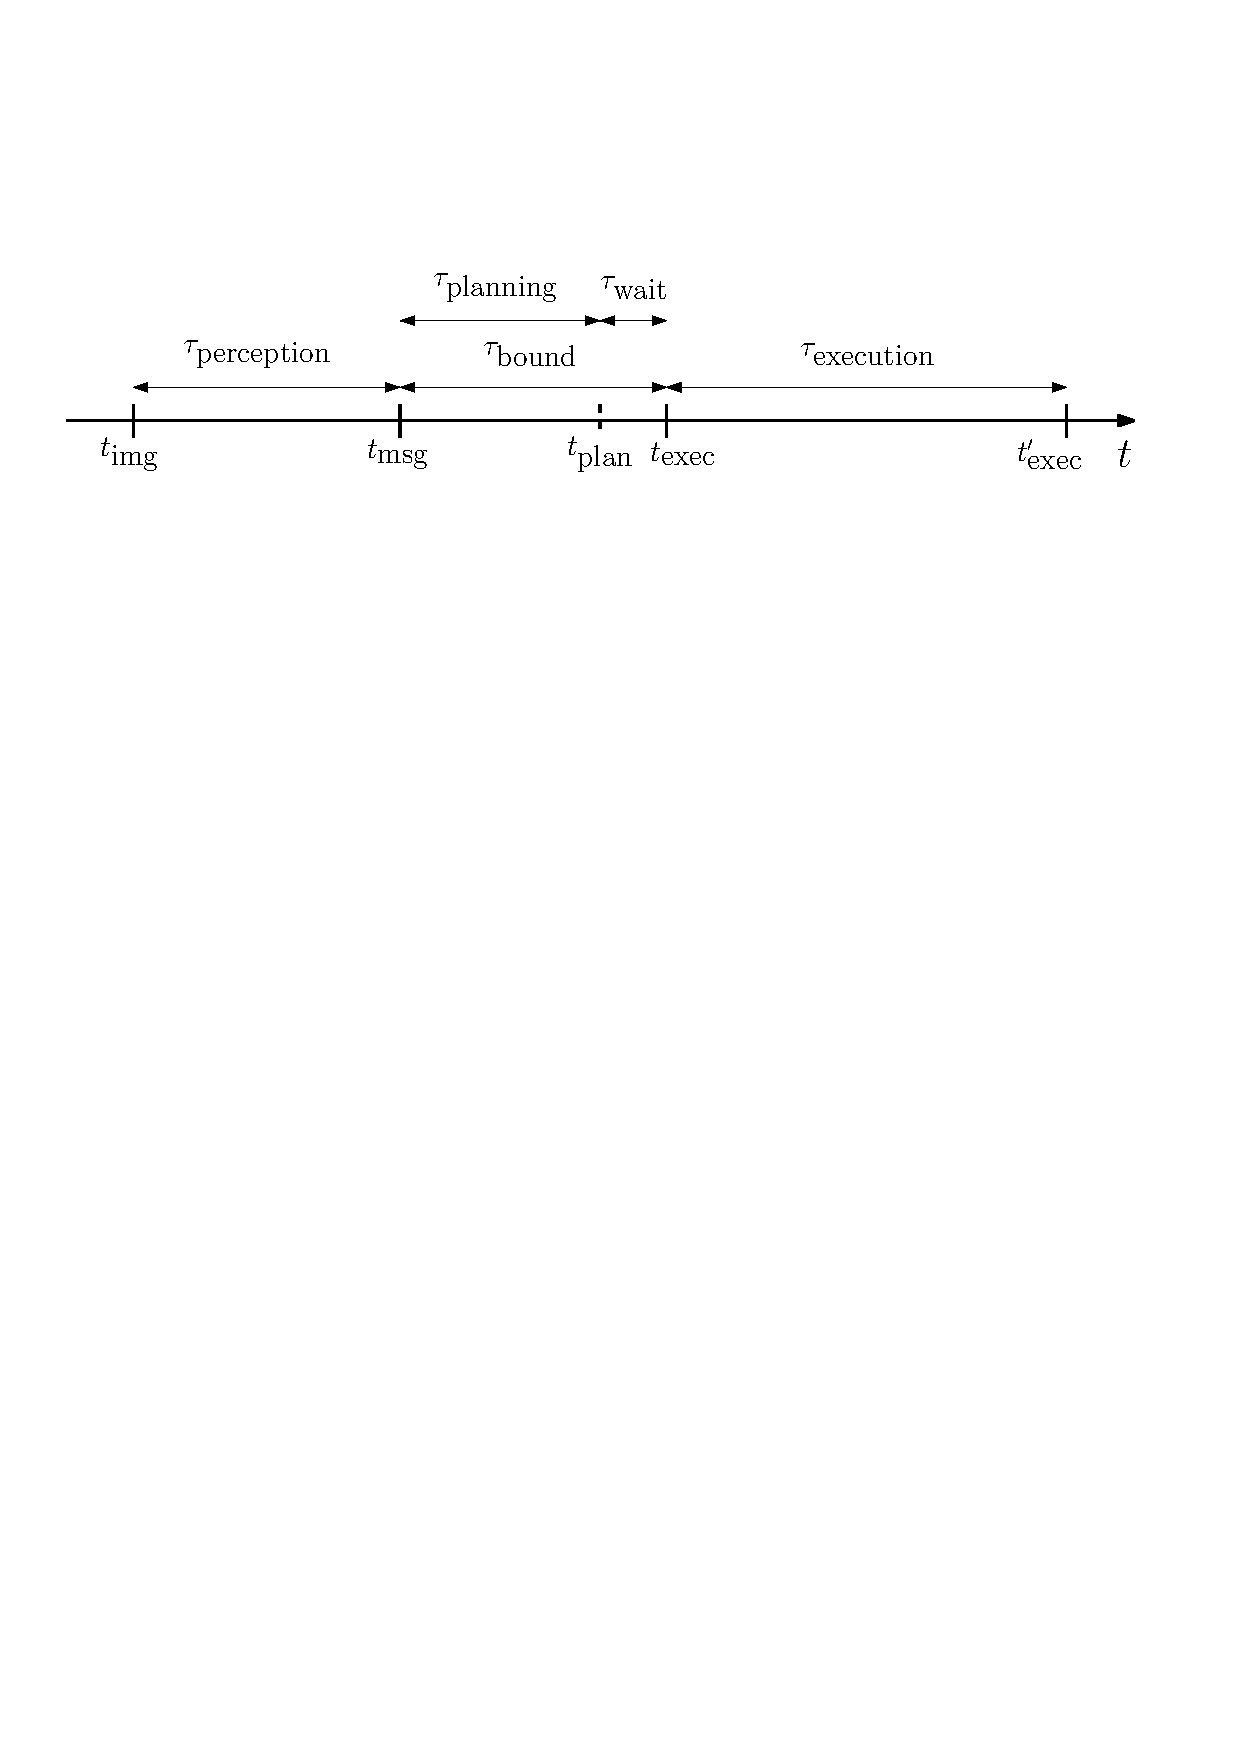
\includegraphics[width=0.5\textwidth]{figs/timeline.pdf}
    \caption{The figure shows the different time triggers on a timeline (increasing left to right) that are used for one ``perception" $\rightarrow$ ``planning" $\rightarrow$ ``execution" cycle while the object moves on the converyor from left to right.
    1.~$t_{\textrm{img}}$ is when the robot captures the image (point cloud) of the object. 
    2.~$t_{\textrm{msg}}$ is when the robot finds the pose estimate (in $\tau_{\textrm{perception}}$) and starts planning. 
    3. $t_{\textrm{plan}}$ is when the plan is computed. Note that our planner guarantees that $t_{\textrm{plan}}$ will be computed within the bound $\tau_{\textrm{bound}}$. 
    4. After $t_{\textrm{plan}}$ the robot waits for $\tau_{\textrm{wait}}$
    5. At $t_{\textrm{exec}}$, the robot starts executing the plan. Note that the goal $g$ that the planner plans for is not for the object pose at $t_{\textrm{img}}$ but its forward projection in time to $t_{\textrm{exec}}$ to account for $\tau_{\textrm{perception}}$ and $\tau_{\textrm{bound}}$.
    6. During the execution time $\tau_{\textrm{execution}}$, if we the robot computes an updated pose estimate, the execution is preempted and the cycle repeats.
    }
    \label{fig:tl}
\end{figure}

\begin{figure}
    \centering
    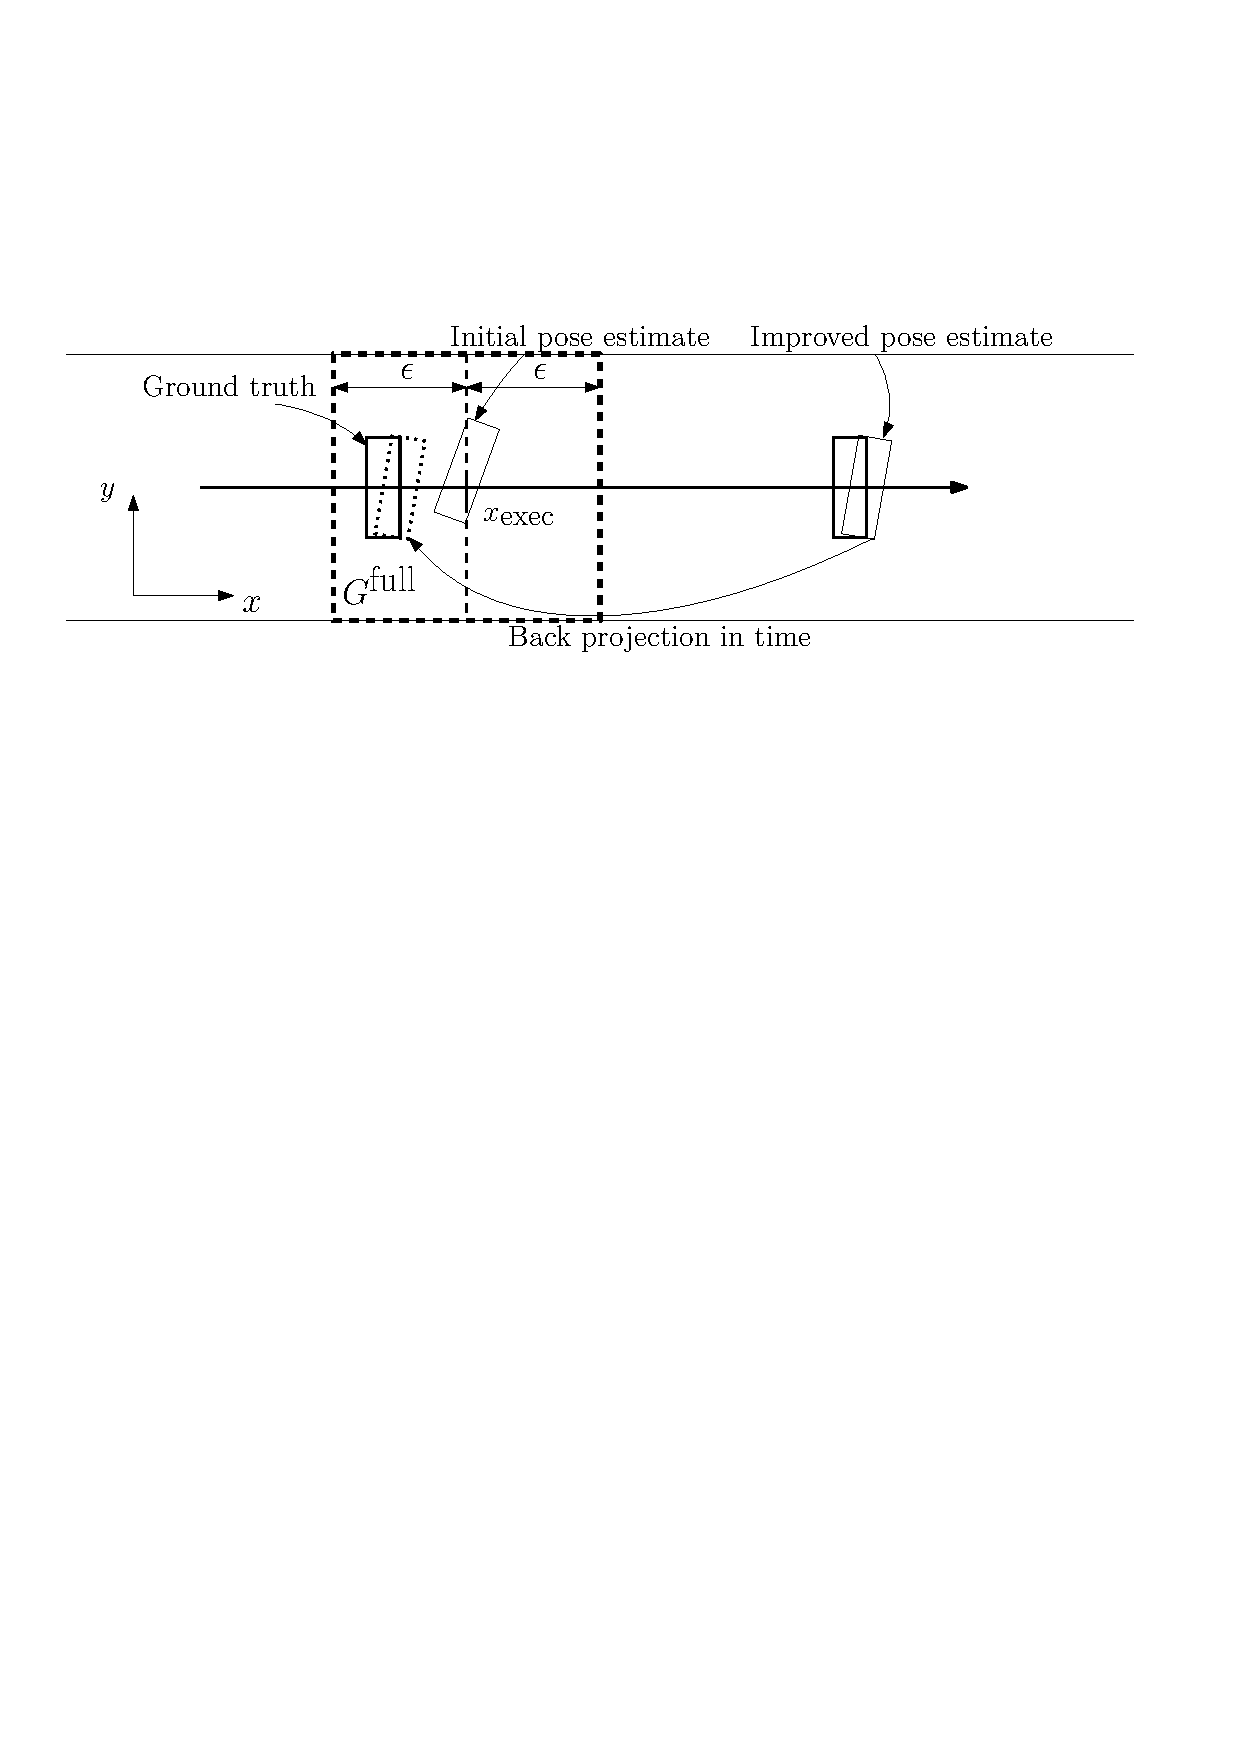
\includegraphics[width=0.5\textwidth]{figs/pose_error.pdf}
    \caption{
    The figure illustrates how we pick $G^{\textrm{full}}$ and how the perception errors are handled in the planning framework. The figure shows the top view of a conveyor belt with the sugar box moving from left to right.
    $G^{\textrm{full}}$ is selected such that the system can handle any arbitrary pose~$(x,y,yaw)$ of the object and also account for a bounded error in the pose estimates.
    $G^{\textrm{full}}$ contains all possible $y$ positions of the object as well as all $yaw$ angles. 
    Along the $x$-axis it contains a window of size $\pm \epsilon$ centered along a position $x_{\textrm{exec}}$.
    $x_{\textrm{exec}}$ is a fixed position that we use to plan for any incoming object for the first planning cycle no matter where the robot first sees the object, but it must be no farther than $x_{\textrm{exec}}$.
    %
    In the shown example, the thick and the thin solid rectangles show the ground truth and estimated poses respectively at two time instances in the life time of the object.
    The first plan is generated for the pose shown at $x_{\textrm{exec}}$. During execution, the robot receives an improved estimate and has to replan for it. At this point we back project this new estimate in time using the known speed of the conveyor and the time duration between the two estimates. This back-projected pose (shown as the dotted rectangle) is then picked as the new goal for replanning. Now under our assumption that the estimate will be within the $\pm \epsilon$ window along $x$ dimension, it will always lie within $G^{\textrm{full}}$ and as $G^{\textrm{full}}$ contains all ($y, yaw$), it can handle the errors along those dimensions.
    }
    \label{fig:pe}
\end{figure}

\subsection*{Our Algorithm}
\begin{itemize}
    \item Preprocessing: total preprocessing time, memory consumption, total trajectories stored, total states for which Alg.~\ref{alg:2} was called, mean time for \textsc{PlanPath}() function 
    \item Query (Planning): mean planning time, mean execution time, success rate 
    \item Query (Replanning): success rate for experiments with varied number of replanning requests

In order to pick a known object moving object along the conveyor, we need a method to estimate its 3-DoF pose at various locations across the conveyor. For this purpose we created an ICP based pose estimation strategy that uses the known 3D model of the object and initial pose estimate obtained after pre-processing the input point cloud. The estimation is performed at every received at every frame. The first step in the pre-processing involves removal of all points that lie outside the known conveyor region, essentially only preserving points corresponding to the object of interest. This is followed by statistical outlier removal in order to remove any points that have been left in scene after the first step. In the final step, we compute the mean of the points left and use that as an initial translation estimate for ICP. The rotation estimate is applied in a way that it places the object parallel to its direction of motion along the conveyor. The object’s 3D model is transformed with this initial estimate, creating a point cloud and ICP refinement is performed between this point and the pre-processed observed point cloud. The resulting transform is concatenated with the initial estimate to return the final predicted pose. For speeding up ICP, we downsample all point clouds to a leaf size of 1.5cm.
\end{itemize}